\newpage
\section{Implementacja}
%\vspace{1cm}
    \subsection{Interfejs użytkownika}\label{interface}
    Interfejsy użytkownika w aplikacjach na system operacyjny Android są standardowo tworzone za pomocą języka znaczników XML, przy czym same znaczniki są generowane przez odpowiednie biblioteki 
    (wbudowane lub zewnętrzne). Podstawowym elementem interfejsu jest Widok (ang. \emph{View}), bazowa klasa każdego interaktywnego komponentu interfejsu użytkownika. Widoki pogrupowane są w Grupy 
    Widoków (ang. \emph{ViewGroup}) zwane zazwyczaj Layoutami~\cite{VIEW}. 

    Za wizualną oprawę aplikacji odpowiedzialne są głównie elementy interfejsu oferowane przez Material Design. Jest to zbiór elementów interfejsu i język designu stworzony i rozwijany przez Google 
    z myślą o tworzeniu aplikacji mobilnych. W procesie tworzenia aplikacji wykorzystane zostały takie elementy jak Bottom App Bar, pozwalający na wygodną nawigację pomiędzy ekranami aplikacji, czy
    Card View, zapewniające elegancki sposób wyświetlania elementów list. Warto przyjrzeć się też elementom o nazwie Chip~\cite{CHIPS}. Są to małe składniki interfejsu, na które składa  
    się przede wszystkim obwódka oraz wyświetlany w jej wnętrzu tekst. Z pozoru mogą wydawać się szczególnym rodzajem zwykłego przycisku, ale różni je stojąca za nimi idea projektowa. Przycisk jest elementem, od którego 
    oczekiwana jest konsekwencja, zarówno wizualna, w wyglądzie, jak i w działaniu, a więc  uruchamianie oczekiwanej przez użytkownika akcji. Chip tym różni się od przycisku, że jego cel jest bardziej dynamiczny --- 
    często reprezentuje on grupę elementów interaktywnych~\cite{CHIPS_GL}. Chipy można podzielić na cztery grupy: 
    
    \begin{itemize}
    	\item 
    pomocnicze (ang. \emph{Assist}), najbliższe w swoim działaniu przyciskom, które powinny pojawiać się w
    interfejsie dynamicznie i kontekstowo;
    \item filtrujące, które za pomocą zmiany koloru i pojawienia się ikony obrazują wybór użytkownika;
    \item  wprowadzające (ang. \emph{Input}), które zastępują dyskretne dane wprowadzone przez;
    użytkownika, 
    \item sugerujące (ang. \emph{Suggestion}), mające graficznie reprezentować dynamicznie generowane podpowiedzi. 
        \end{itemize}

    
    W aplikacji mobilnej zastosowane zostały Chipy Pomocnicze, w konstrukcji przejrzystego
    interfejsu komponującego się z wyświetlaną w tle mapą, oraz Filtrujące, zapewniające użytkownikowi responsywny system wyboru kategorii oraz etykiet dla Miejsc. Aplikacje projektowane na system Android 
    posiadają także ujednolicony system tworzenia motywów kolorystycznych. W aplikacji zastosowany został motyw stworzony za pomocą Material Theme Builder, narzędzia wspomagającego poprawny dobór 
    kolorów oferowanego przez Material Design~\cite{THEME}.

    Tworzenie aplikacji na system Android polega także na korzystaniu z rozwijanego przez Google obszernego zestawu bibliotek Android Jetpack~\cite{JETPACK}. Zawiera on w sobie podstawowe 
    komponenty aplikacji mobilnych, takich jak np. Aktywności (pojedynczy ekran interfejsu użytkownika, analogiczny do okna w aplikacji komputerowej), czy biblioteki obsługujące Material Design. Oferuje 
    on także szereg rozwiązań usprawniających projektowanie aplikacji takich jak np. Navigation Component, ułatwiający poruszanie się pomiędzy ekranami aplikacji i oferujący wizualną reprezentację akcji 
    nawigacyjnych, które mogą zostać podjęte przez użytkownika (Rysunek~\ref{jetpack}).

  %  \vspace{1cm}
    \begin{figure}[!ht]%
        \centering
        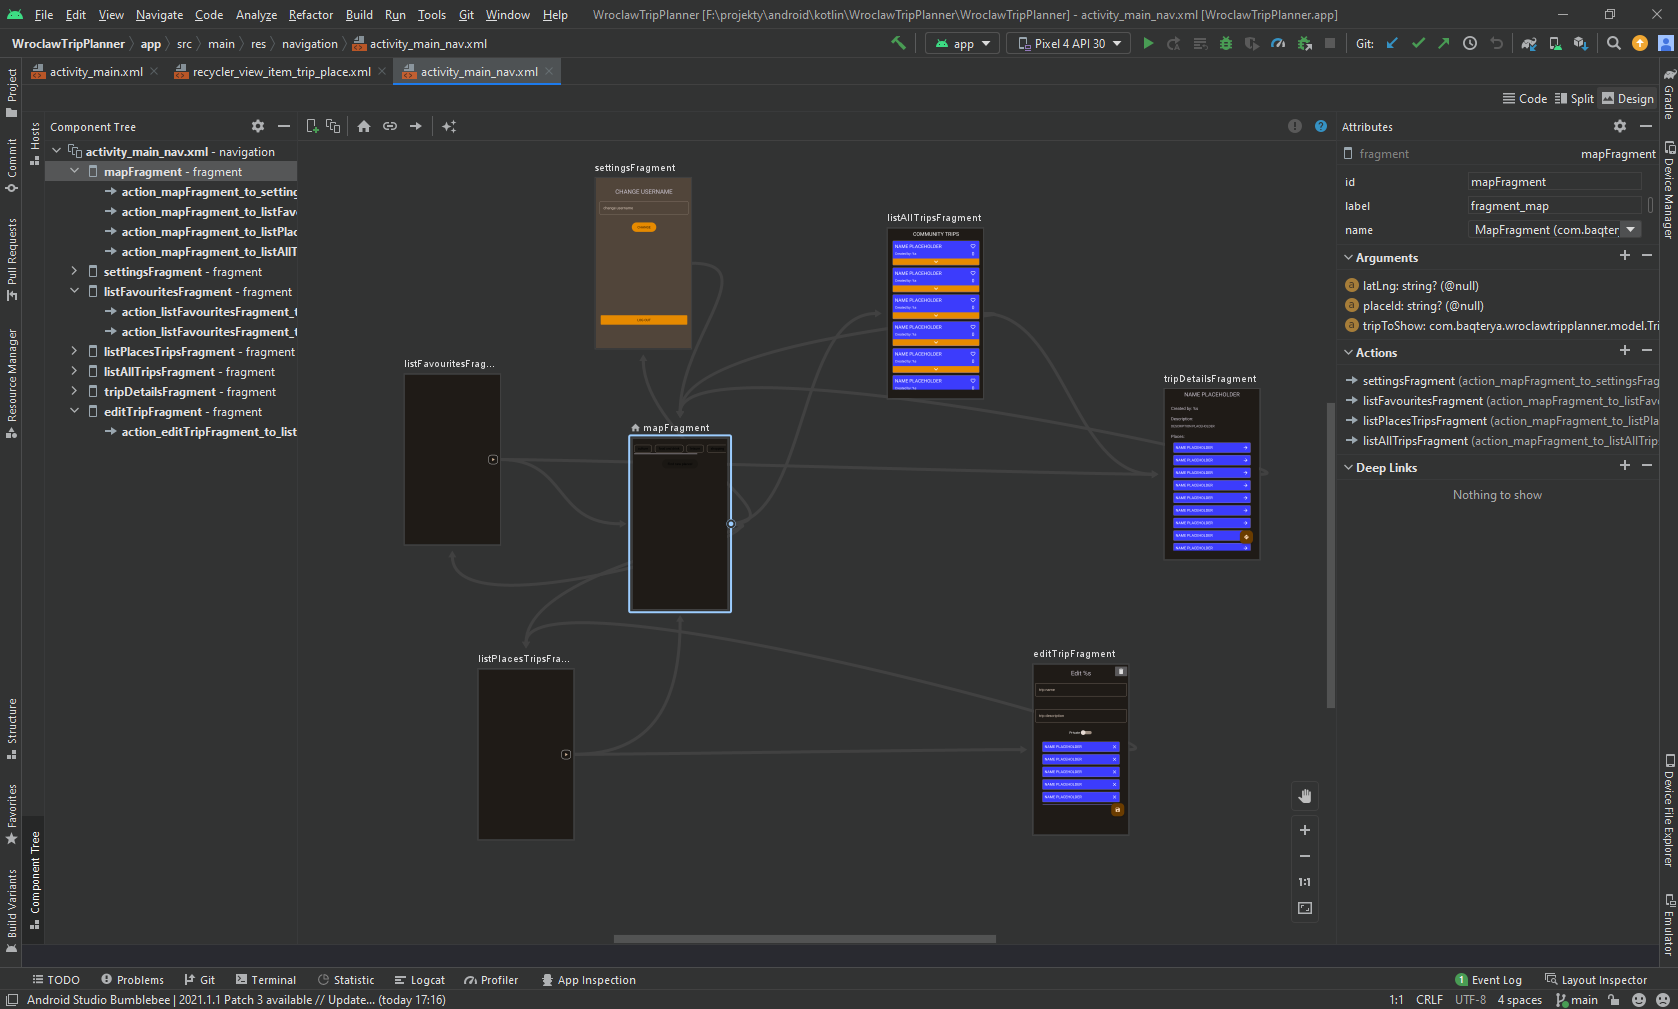
\includegraphics[scale=0.35]{src/jetpack_nav.png}
        \caption{Akcje nawigacyjne reprezentowane na diagramie Naviagtion Component.\label{jetpack}}
        \qquad
    \end{figure} 
  %  \vspace{1cm}

    W odróżnieniu od standardowego stylu tworzenia aplikacji, w którym kod inicjowany jest za pomocą metody \texttt{main()}, aplikacje na system Android wykorzystują Aktywności. Aktywność reprezentuje 
    pojedynczy ekran interfejsu użytkownika, na którym wyświetlane są interaktywne widoki. To w nich zawiera się kod odpowiadający za obsługę wszelkich funkcji aplikacji takich jak np. efekt wciśnięcia
    przez użytkownika danego przycisku, wprowadzenia tekstu itp. Wizualna warstwa Aktywności obsługiwana jest przez plik XML zawierający umiejscowienie i właściwości elementów interfejsu użytkownika.
    Aktywności posiadają określony cykl życia, który określa jej aktualny stan, oraz stan danych zadeklarowanych w konkretnej aktywności (Rysunek~\ref{lifecycle}). Informacja wprowadzona przez 
    użytkownika w jednej aktywności zostanie skasowana z pamięci telefonu w momencie zatrzymania się aktywności, więc twórca aplikacji musi zapewnić poprawny transfer danych pomiędzy nimi. 

  %  \vspace{1cm}
    \begin{figure}[!ht]%
        \centering
        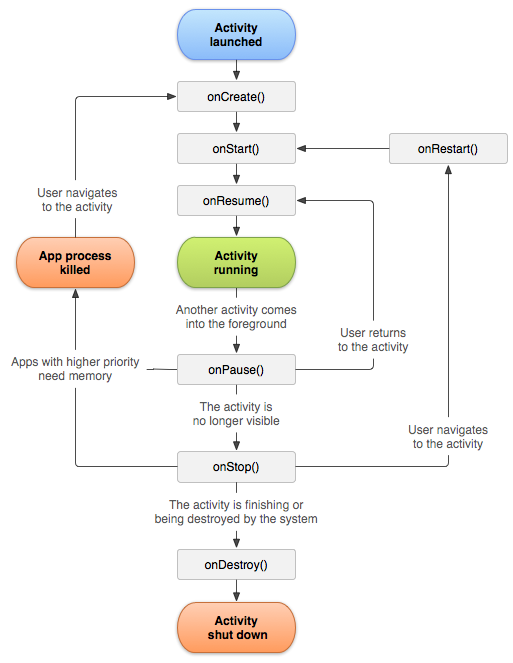
\includegraphics[scale=0.45]{src/activity_lifecycle.png}
        \caption{Cykl życia Aktywności~\cite{LIFECYCLE}.\label{lifecycle}}
        \qquad
    \end{figure} 
%    \vspace{1cm}

%\newpage
    Kolejnym istotnym elementem interfejsu użytkownika jest klasa Fragment, stanowiąca część interfejsu przeznaczoną do wielokrotnego użytku. Każdy fragment musi zawierać się w aktywności, natomiast każda aktywność 
    może zarządzać dowolną liczbą fragmentów. Są one łatwe w modulacji i pomagają dyskretnie dzielić interfejs użytkownika. W trakcie działania aktywności fragmenty przechodzą swój własny, analogiczny, 
    ale oddzielny cykl życia. Dużą zaletą korzystania z fragmentów jest szerokie wsparcie dla aplikacji opartych na fragmentach. Dobrym przykładem jest wspomniany wcześniej Navigation 
    Component. Pojedynczy komponent tego typu implementowany jest w konkretnej aktywności. Opisana tu aplikacja zawiera w sobie dwie aktywności: jedną odpowiadającą za procesy logowania i rejestracji oraz drugą, 
    zawierającą główną, użytkową część aplikacji. Na przykład w pierwszej z nich użytkownik może nawigować pomiędzy trzema fragmentami odpowiedzialnymi za wyświetlenie ekranu powitalnego, ekranu logowania,
    oraz ekranu rejestracji. Z punktu widzenia użytkownika nie ma różnicy pomiędzy użyciem fragmentu lub aktywności, jednak dla twórcy aplikacji rozwiązanie to oferuje znacznie większą elastyczność i wygodę.

